\chapter{The algorithm}\label{cap:Algorithm}
We present here the algorithm we developed for data association with bearing only sensor.

The program takes as input a file that has a line for each step of the trajectory.
Each line specifies:
• The rototranslation with respect to the previous step (x, y, theta)
• a list of the measurements acquired in this step.

The basic idea is that, at each step, the algorithm iterates over all the observations associated with the considered position and tries to associate them with observations from the previous step, determining if each observation should be \textbf{queued} to one of the previous tracks or it should be associated to a new landmark.

A landmark is considered \textbf{confirmed} when it has at least a certain number of associated observations.

The \textit{track}, to which we will often refer in this chapter, is actually a landmark. When new observations are added to the track, the landmark position is re-estimated and the track is propagated to the next step.
When, on the contrary, no new observations are associated to the track, it is not propagated, and the landmark itself is either pruned or kept (depending on the fact that it had been confirmed or not).

Going on with the trajectory, the algorithm creates a graph, putting in it new poses and landmarks.

Every time a certain number of steps has been performed, the graph is optimized according to the edges created up to that moment.

After the trajectory evaluation is terminated, the optimized poses can be used to re-initialize the algorithm, keeping the bearing measurements unchanged, so to re-associate the data. This is known as \textit{Expectation Maximization}.

In section \ref{sec:issues} we illustrate the problems we had to face, and how we dealt with them.
After that, in section \ref{sec:pseudocode} there is a pseudo-code of the developed algorithm.

\section{Issues}\label{sec:issues}
\subsection{The main problem: vague observations}
Using a bearing only sensor involves a big problem: an observation is not enough to estimate the position of a landmark.
From an observation associated with a robot position we can only determine a line (actually an half line) where the landmark may be.
This is a problem because next step observations can't rely on the estimated position of the landmark for determining correspondances.

The developed algorithm deals with this problem distinguishing two cases (see figure \ref{fig:observation_association}):
\begin{enumerate}
  \item The landmark already has an estimated position.
  \item A position has not been estimated for the landmark. (Usually happens when the landmark has been seen only once)
\end{enumerate}
\begin{figure}[htbp]
  \centering
    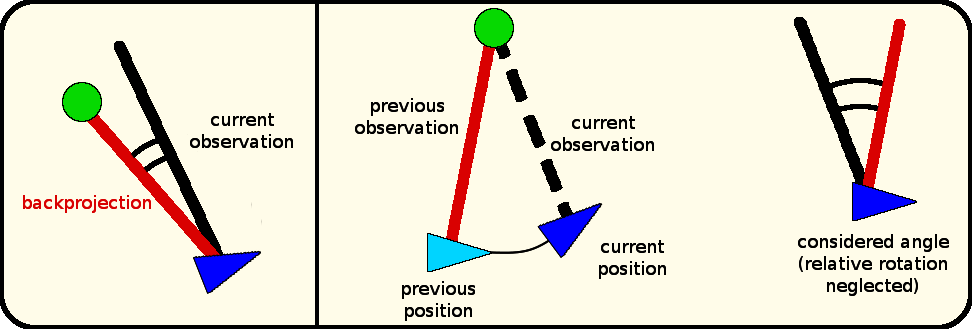
\includegraphics[width=0.8\textwidth]{images/observation_association.png}
  \caption{The two possible situations. The drawn angles are those to be evaluated.}
  \label{fig:observation_association}
\end{figure}
In the first case, the estimated position is backprojected on the robot pose, and the resulting angle is compared to the current observations.

In the second case, an assumption is made: given that the captures are ``close'', the sensed bearing for the same landmark should have remained similar between two consecutive steps. The comparation is then done only with the previous angle (of course after considering positions relative rotation).

\subsection{More than a close track}\label{subsec:twotracks}
It can happen that the observation we are evaluating is close to two of the tracks. There is of course a track that is ``closer'' than the other, but they are both inside a certain threshold.\footnote{We actually defined a threshold for the closer and another threshold for the second closer.}
In this case, we simply start a new track with the new observation.

\begin{figure}[htbp]
  \centering
    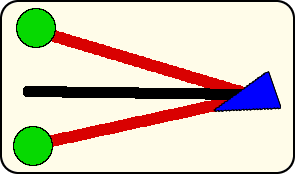
\includegraphics[width=0.3\textwidth]{images/uncertainty1.png}
  \caption{Two close observations. How to choose?}
  \label{fig:uncertainty1}
\end{figure}

To understand the sense of this choice, it is the case to highlight the importance of avoiding wrong associations.
Since we can only rely on the bearing for the landmarks position estimation, a wrong association can cause the graph to explode when optimizing.
This is then wiser, where possible, to avoid every source of uncertainty.
A pessimistic approach will possibly discard some good informations, but will be more reliable.

\subsection{Two observations for the same track}\label{subsec:twoobservations}
In section \ref{subsec:twotracks} we have seen that an observation could be close to two tracks.
We now face the dual problem: it can happen that two of the current observations are close to the same track.

\begin{figure}[htbp]
  \centering
    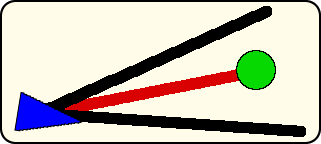
\includegraphics[width=0.3\textwidth]{images/uncertainty2.png}
  \caption{Two new observations are both close to the same track.}
  \label{fig:uncertainty2}
\end{figure}

Just like before, we cannot risk to associate a landmark with wrong measurements.
Moreover, it is obvious that a single landmark shouldn't generate two measurements.
Following the idea that not knowing is better than thinking wrong, we don't add either of the two observations to the track.
Anyway, if the landmark had been \textit{confirmed} (I.E. it is considered reliable), its corresponding track  is propagated to the next trajectory step.

\subsection{Further robustness}
Even with the precautions explained in sections \ref{subsec:twotracks} and \ref{subsec:twoobservations}, it can still happen that a wrong association is generated. In order to deal with this problem, the effect of edges in the optimization steps is limited via the use of the so called \textit{robust kernels}.
These are filters that impose a saturation threshold, over which the constraint effect can't grow anymore.

\section{Pseudo-code}\label{sec:pseudocode}
In this section, a pseudo-code for the algorithm is given.

First of all, some pseudo-structures.
\begin{itemize}
  \item RobotPosition: this represents a pose, and will contain:
    \begin{itemize}
      \item Coordinates and orientation (x,y,theta).
      \item A set of Observations.
    \end{itemize}
  \item Observation: this represents a measurement. It will be defined by:
    \begin{itemize}
      \item A reference RobotPosition.
      \item A bearing value.
    \end{itemize}
  \item Landmark: this represents a landmark, and is also used to propagate tracks. It will consist of:
    \begin{itemize}
      \item Coordinates (x,y).
      \item A set of references to Observations (all the observations that have been associated to this landmark)
      \item Confirmed status. It will be set to true when the landmark has been seen enough times.
    \end{itemize}
\end{itemize}

And here is the algorithm:
{\footnotesize
  \lstset{language=C}
  \begin{lstlisting}[frame=shadowbox,breaklines]
    definitions:
    	OPTIMIZE_EVERY	// every time this number of steps has been performed, an optimization sequence is made
        MIN_ANGLE_DIST	// angles threshold for observations association
        SECOND_MIN_ANGLE_DIST	// P x MIN_ANGLE_DIST, P>=1
    
    global variables: 
    	landmarks_list	// list where landmarks are inserted
        graph	// the graph to be used for optimization
        
    // This function manages the algorithm iterations.
    // 'steps' is the sequence of steps, each with the relative transformation with respect to the previous step and a set of observations.
    algorithm_launcher(steps)
    {
      // 'previous_observations' and 'propagate_observations' are lists used to keep track step after step of the observed landmarks
      previous_observations = new empty Landmarks list;
      propagate_observations = new empty Landmarks list;
      
      int loop_count = 0;	// increases at every step, is set to 0 when optimization is performed
      
      for each step
        loop_count ++;
      	current_position = compute the new position appending the new step to the previous one;
        current_position.observations = step.observations;
        
        // the observations propagated from the previous step are moved to the specific list
        previous_observations = propagate_observations;
        clear propagate_observations;
        
        propagate_observations = tryToUnderstand(current_position, previous_observations);
        
        if loop_count > OPTIMIZE_EVERY
        	loop_count = 0;
                populate the graph with new landmarks nodes and edges;
                graph.optimize();
        
      // end of 'for each step'
      
      // last optimization
      populate the graph with new landmarks nodes and edges;
      graph.optimize();
      
      // expectation maximization
      in case it is needed/required_by_the_user
      	steps = compute relative transformations from the optimized positions;
        algorithm_launcher(steps)	// rerun the algorithm
    }
    
    
    // this is the actual data association function
    // returns a Landmark list containing the tracks to be propagated to the next step
    // REMEMBER that 'tracks' are just 'landmarks', hence the term is often used interchangeably
    tryToUnderstand(current_pose, previous_observations)
    {
      // prepare structures
      list<Landmark> propagate;	// list used to propagate tracks to the next step.
      
      double expected[previous_observations.size()];	// an array of doubles with a value for each of the previous observations
      
      int associations[current_pose.observations.size()]	// an array with as many integers as the measurements in the current pose.
      
      // populate 'expected' with the angles where we expect to see the landmarks that have been propagated from the previous step
      for each landmark 'lmark' in previous_observations
      	// first case
      	if the landmark has an estimated position
          expected.add(backprojection(lmark, current_pose));
        else  // second case
          prev_measure = extract last measured angle for the landmark;
          expected.add(prev_measure - relative_rot);	// relative_rot is the rotation performed from the previous step
      
      // at this point, expected contains the angles to be compared with new observations
      
      // try to associate new observations to previous tracks
      for each observation 'obs' in current_pose.observations
        
        // compute the angle distances from the 'expected' angles 
        double distances[previous_observations.size()];
        distances <- computeDistances(obs.bearing, expected);
        // 'distances' now contains the ``distance'' of the current observation from each of the expected values
        
        // 'closer' and 'second_closer' will be used to identify the two most likely tracks for this observation to be associated
        int closer;
        int second_closer;
        
        closer =  index of min(distances);
        second_closer = index of min_i(distances, i!=closer);
        
        if distances[closer] < MIN_ANGLE_DIST	// the closer expected angle is close enough
        	
        	//first case
                if distances[second_closer] > SECOND_MIN_ANGLE_DIST
                	// the second closer angle is far enough: no ambiguity.
                        // store information that this angle should be associated to the landmark that generated the considered expected value
                        associations[obs] = closer;
                        // note that the observation is not added to the track yet, because there ould still rise ambiguity with 
                else
                	// the second closer angle is lower than its threshold: there is ambiguity
                        associations[obs] = -1	// just an invalid value.
                        
        else	// distances[closer] > MIN_ANGLE_DIST: this new observation is far from all the existing tracks
        	associations[obs] = -1	// just an invalid value.
      
      // end of 'for each observation...'
      
      // at this point associations[i] contains, which is the track to which the new i-th observation should be associated. If there are no associable tracks or there are more than one, this value is -1 (invalid)
      
      // next step: determine another kind of ambiguity: when two new observations ask to be associated to the same existing track
      
      bool has_new_obs[previous_observations.size()];
      // a boolean for each track
      // has_new_obs[i] will be set to true if at least one new observation is associable to the i-th track
      
      bool ambiguous[previous_observations.size()];
      // a boolean for each track
      // ambiguous[i] will be set to true if more than one observation is associable to the i-th track
      
      // initialize the two arrays to all false values
      has_new_obs <- false;
      ambiguous <- false;
      
      // look for ambiguities
      for each observation 'obs' in current_pose.observations
      	int value = associations[obs];	// value is the index of the track to be associated
        
        if value != -1
        	if has_new_obs[value] == false
                	has_new_obs[value] = true
                else
                	ambiguous[value] = true
                        
      // at this point ambiguous[i] is true if the i-th track has two or more potential new observations
      // add non-ambiguous new observations to the corresponding track, and create new tracks for the newly observed unassociated observations
      
      for each observation 'obs' in current_pose.observations
      	track_index = associations[obs];
      	if track_index != -1
        	if ambiguous[track_index] == false	// obs can be tailed to the track
        	        selected_track = previous_observations[track_index];
                        selected_track.addObservation(obs);
                	re-estimate landmark position;
                        check if the landmark should be set to 'confirmed', and in case set it;
                        propagate.add(selected_track);
                else
                	// obs can't be tailed to the track, because there is ambiguity
        else
        	// this observation has been considered a new track
                Landmark lm = new Landmark();
                lm.addObservation(obs);
                landmarks_list.add(lm);	// add the landmark to the overall landmarks set
                propagate.add(lm);	// add the landmark to the tracks to be considered in the next step
    
      
      // now re-scan all the tracks from previous step, and if needed prune them (kill the landmark).
      for each track 'tr' in previous_observations
      	if has_new_obs[tr] == false
        	// we expected to see this landmark, but we didn't so we have two cases:
                if tr.confirmed == true
                	// we trust this landmark
                else
                	// this track is too young
                        landmarks_list.remove(tr);	// delete the landmark from the overall landmarks set
        
        else
        	// some new observations were close to this track
                if ambiguous[tr]
                	// this track was not enhanched, because two or more observations were close to it
                        // check it's reliability
                        if tr.confirmed == true
                        	// it is the case to keep tracking this valuable landmark
                                propagate.add(tr);
                        else
                        	// this 'young' track is already giving problems... just remove it
                                landmarks_list.remove(tr);
                
      
    return propagate;
    }
  \end{lstlisting}
}


